\pdfoutput=1
\documentclass[11pt,a4paper]{article}
\usepackage{abhijit-research}
\renewcommand{\PaperCode}{P16}
\renewcommand{\PaperKind}{RESEARCH PAPER}
\renewcommand{\PaperVersion}{VERSION 1.1}
\renewcommand{\PaperDate}{AUGUST 2026}
\renewcommand{\PaperTitle}{Adaptive Predictive Systems}
\renewcommand{\PaperSubtitle}{Native Representation Repair}
\renewcommand{\PaperFullTitle}{Adaptive Predictive Systems with Native Representation Repair}
\renewcommand{\PaperShortTitle}{Adaptive Predictive Systems}
\renewcommand{\PaperKeywords}{predictive state; representation repair; provenance; active learning; adaptive systems; continual learning}
\renewcommand{\PaperClassification}{The finite repair mechanisms and supplied benchmark are executable. The full hybrid architecture is a research design whose performance must be established by independent evaluation.}
\renewcommand{\PaperCitation}{Singh, Abhijit. 2026. \textit{Adaptive Predictive Systems with Native Representation Repair}. Research manuscript, version 1.0.}
\begin{document}
\MakeResearchTitle
\MakeResearchContents
\MakeResearchAbstract{%
A model-agnostic computational architecture is proposed for systems that can detect when their current state representation is insufficient, acquire a separating observation, refine the representation conservatively, verify the change by ablation and restoration, and continue without losing source provenance. The architecture combines a recurrent long-context backbone, sparse attention, routed specialist modules, a source-addressed event graph, a minimal predictive-state compiler, relation-aware disagreement routing, active experiment planning, future-tested memory compression, and a validated schema-repair engine. A collision benchmark spanning provenance, time, role, relation, tool version, and history depth raises exact continuation from 6/12 under a coarse report to 12/12 after essential-coordinate repair. The large-scale performance claim remains an evaluation target. A new 36-relation benchmark tests detection, separator acquisition, conservative repair, ablation, and restoration.
}
\section{Objective}
The architecture targets a structural failure of fixed-state systems: two histories may receive one current representation although a later allowed intervention requires different actions. More computation inside the same quotient cannot restore a distinction that the quotient erased. The system must be able to detect representation failure, acquire a separator, refine its state conservatively, and continue from the repaired representation.

\section{System state}
At step $t$ carry
\begin{equation}
\mathcal S_t=(z_t,Q_t,\Pi_t,B_t,\Gamma_t,\Lambda_t,K_t),
\end{equation}
where $z_t$ is fast working state, $Q_t$ a compiled predictive quotient, $\Pi_t$ an append-only source graph, $B_t$ unresolved future-separating boundaries, $\Gamma_t$ relations among parallel hypotheses, $\Lambda_t$ available interventions, and $K_t$ verified cached transitions.

The primary prediction is
\begin{equation}
P(y_t,S_{t+1},\Delta_t\mid S_t,a_t,\Pi_t),
\end{equation}
not merely a distribution over the next symbol. Every answer is coupled to its successor state, source support, scope, uncertainty, counterconditions, and unresolved residuals.

\section{Hybrid computation}
A practical system combines:
\begin{enumerate}
\item selective recurrent state-space blocks for long-context throughput;
\item sparse attention for exact local and retrieved interactions;
\item routed expert modules for semantic, causal, formal, spatial, and operational tasks;
\item graph message passing over provenance and hypothesis relations;
\item an explicit predictive-state compiler and boundary detector.
\end{enumerate}

\begin{figure}[H]\centering
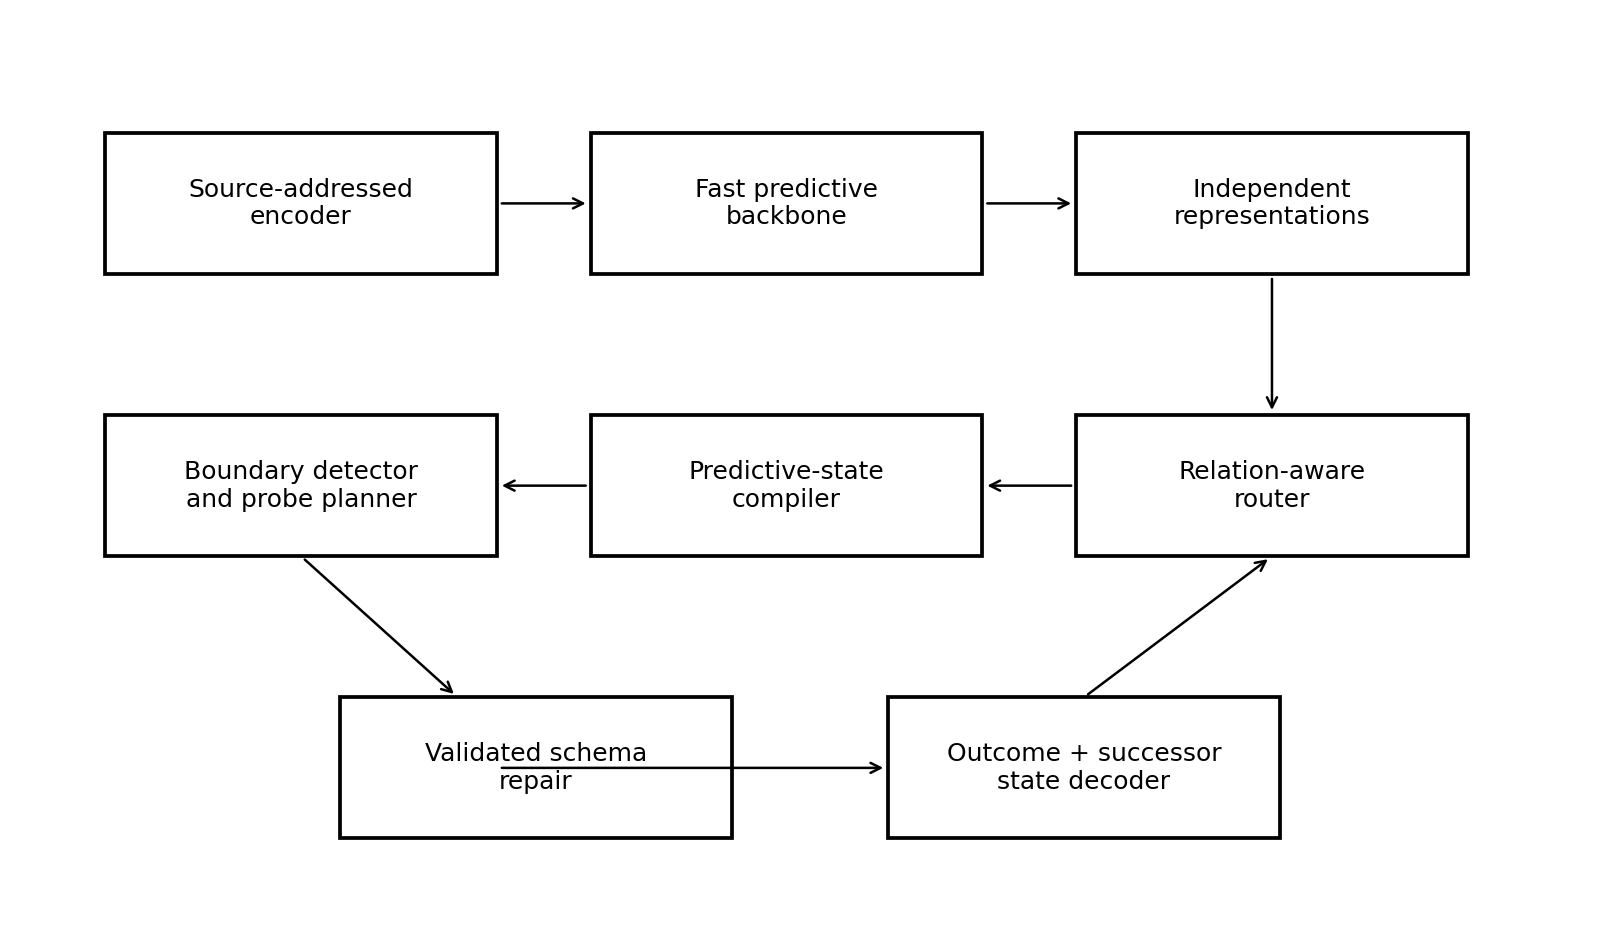
\includegraphics[width=.94\linewidth]{figures/p16_architecture.png}
\caption{Reference architecture for source-preserving predictive repair.}
\end{figure}

\section{Predictive-state compiler}
For history $h$ and intervention family $\Lambda$, define the approximate continuation signature
\begin{equation}
\Sigma_\Lambda(h)=\{P(Y_{1:H}\mid\operatorname{do}(\lambda),h):\lambda\in\Lambda\}.
\end{equation}
Merge histories only when the divergence of their signatures is below a declared tolerance. The compiler seeks the smallest state preserving the futures for which the system is responsible.

\section{Boundary detection and experiment planning}
A boundary is active when one report fibre contains future-distinct histories. Choose a separating operation by
\begin{equation}
\lambda^*=\arg\max_{\lambda\in\Lambda}
\frac{\mathbb E[\text{future separation from }\lambda]}{\operatorname{cost}(\lambda)}.
\end{equation}
A separator can be a clarifying question, retrieval, code execution, theorem check, simulation, new sensor reading, or controlled counterfactual.

\section{Validated schema repair}
A new coordinate is admitted by
\begin{equation}
\widetilde U(h)=(U(h),\eta(h)),\qquad\pi_1\widetilde U=U.
\end{equation}
Admission requires source provenance, improvement on frozen continuation tests, matched ablation, restoration, backward compatibility, and rollback. A written memory or metadata field that never changes a later operation is not a repair.

\section{Independent representations and relation-aware routing}
Upper representations are trained with partially decorrelated error structures. A relation model observes predictions, uncertainty, source dependence, agreement, contradiction, and prior contact performance. It may select, synthesize, preserve alternatives, or request a separator. The source-reported 97.78 percent result motivates relation-aware routing; the failed higher-arity rescue prevents the architecture from treating relation count as a universal solution.

\section{Future-tested memory compression}
Working memory, predictive-state memory, exact episodic provenance, and unresolved-boundary memory are separate. A feature can be deleted only when its removal leaves the declared future distribution invariant. The chronological 13-channel study is a direct regression test for this rule.

\section{Training objective}
A native objective can combine
\begin{equation}
\mathcal L=\mathcal L_{\rm seq}+\alpha\mathcal L_{\rm world}+\beta\mathcal L_{\rm closure}
+\gamma\mathcal L_{\rm source}+\delta\mathcal L_{\rm relation}
+\eps\mathcal L_{\rm repair}+\mu\mathcal L_{\rm verify}+\nu\mathcal C_{\rm compute}.
\end{equation}
The closure loss penalizes merged states with divergent future signatures; a complexity penalty prevents retention of every historical difference.

\section{Collision benchmark}
The supplied reference benchmark contains six collision families: source identity, temporal phase, causal role, relation compatibility, tool version, and history depth. Twelve source cases share six coarse reports. A first-answer coarse baseline is correct on 6 of 12. The essential-coordinate compiler selects coordinates $(0,2)$ and raises exact continuation to 12 of 12. Removing either selected coordinate reintroduces a collision. Two benchmark tests pass.

\begin{table}[H]\centering
\caption{Reference collision benchmark.}
\begin{tabular}{lrr}
\toprule
system & correct & total\\\midrule
coarse report baseline & 6 & 12\\
repaired predictive state & 12 & 12\\
\bottomrule
\end{tabular}
\end{table}

\section{Serving policy and speed}
Routine queries use a fast path with cached predictive states, few active experts, and early exit. Deep computation is activated by disagreement, source conflict, long-horizon planning, or a detected boundary. Schema repair is rarer still and runs only after evidence shows that the state vocabulary itself is insufficient. Speed therefore comes from minimal future-sufficient states and conditional escalation, not from treating every query as maximal search.

\section{Nine-state relation-closure benchmark}
A dedicated benchmark instantiates the complete repair cycle on the nine-state carrier. The source has one unit state and four two-sided prime sectors. Its 36 pair relations decompose into eight unit, four return, and twenty-four transverse cells. The coarse reporter erases the side coordinate; the return continuation flips that coordinate while preserving the visible prime label.

A correct system must:
\begin{enumerate}
\item detect that the stationary visible report hides a period-two source recurrence;
\item select the side coordinate as a shortest separator for the declared role-sensitive future;
\item extend the state conservatively from $q$ to $(q,\varepsilon)$;
\item preserve all old value-only answers;
\item fail the role-sensitive task under ablation and recover it under restoration;
\item distinguish the finite static M\"obius classes from the all-prime support-address quotient.
\end{enumerate}
The supplied standard-library verifier checks the finite relation count, return-generator commutation, static false-closure counterexample, support-state update, and Fourier-magnitude control. This is a compact benchmark for native representation repair rather than a claim of general system superiority.

\section{Evaluation}
Standard language, code, mathematics, and multimodal benchmarks remain necessary. Architecture-specific tests should measure:
\begin{itemize}
\item false-closure detection;
\item source collision and role reversal;
\item separator efficiency;
\item oracle-gap routing;
\item representation restoration;
\item dynamic ontology and tool birth;
\item re-entry ablation;
\item memory compaction;
\item time to verified answer.
\end{itemize}
A headline systems measure can report verified task utility per latency and active compute. Raw accuracy must remain visible separately.

\section{Development status}
The predictive quotient and finite repair mechanisms are implemented in the supplied reference code. The large-scale hybrid architecture is a systems design, not a demonstrated frontier model. Performance superiority must be established by independent benchmark comparison. The durable contribution is the representation-repair kernel and benchmark category, not a parameter-count claim.


\section{Complete runtime architecture}
The runtime separates proposal generation from state authority. Replaceable sequence, code, vision, causal, and formal models propose candidate continuations. An explicit kernel controls source addresses, predictive states, intervention planning, verification, and schema migration.

The operative state is
\begin{equation}
\mathcal S_t=(z_t,Q_t,\Pi_t,B_t,\Gamma_t,\Lambda_t,K_t),
\end{equation}
where $z_t$ is fast neural working state, $Q_t$ the compiled predictive quotient, $\Pi_t$ the provenance graph, $B_t$ unresolved boundaries, $\Gamma_t$ relations among parallel hypotheses, $\Lambda_t$ allowed interventions, and $K_t$ verified caches.

\section{Module contracts}
\begin{longtable}{p{.26\linewidth}p{.65\linewidth}}
\toprule
module&required contract\\\midrule
source encoder&content representation plus immutable occurrence address, scope, and parent links\\
predictive compiler&minimal quotient, closure certificate, and counterexample separators\\
relation router&agreement, contradiction, shared-source dependence, prior performance, and branch preservation\\
boundary detector&pairs of histories merged now but divergent under an admitted future\\
probe planner&maximum expected separation per cost, latency, and permission\\
schema engine&conservative coordinate addition, migration, backward projection, and rollback\\
verifier&source, proof, execution, calibration, adversarial, and regression checks\\
decoder&answer, confidence class, source support, successor state, and unresolved conditions\\
\bottomrule
\end{longtable}

\section{Inference cycle}
\begin{verbatim}
encode request with source occurrence
run independent proposal representations
construct relation and provenance graph
compile the smallest future-sufficient state
if no collision:
    use cached fast path and emit successor state
else:
    select the lowest-cost separating intervention
    execute only an authorized probe
    refine the state conservatively
    run ablation, restoration, and backward tests
    commit or roll back the schema change
\end{verbatim}
The answer and successor state are one operation:
\begin{equation}
P(y_t,S_{t+1},\Delta_t\mid S_t,a_t,\Pi_t).
\end{equation}

\section{Relation-aware routing}
Independent high-level representations are deliberately not forced into complete agreement. The relation model observes predictions, confidence, source overlap, contradictions, and past contact performance. It may select one proposal, synthesize compatible proposals, preserve incompatible branches, or request a separator. The 97.78\% held-out result motivates this relation layer, while the failed higher-arity rescue prevents the assumption that more experts automatically solve the remaining cases.

\section{Future-tested memory}
Working memory, minimal predictive state, exact episodic provenance, and unresolved-boundary memory remain separate. A feature is compressed only when its ablation leaves every declared future distribution unchanged. The chronological 13-channel restoration supplies a direct regression test: present reconstruction was not sufficient to justify deletion.

\section{Training objective and curriculum}
The objective is
\begin{equation}
\mathcal L=\mathcal L_{\rm sequence}
+\alpha\mathcal L_{\rm intervention}
+\beta\mathcal L_{\rm false\ closure}
+\gamma\mathcal L_{\rm provenance}
+\delta\mathcal L_{\rm relation}
+\varepsilon\mathcal L_{\rm repair}
+\mu\mathcal L_{\rm verification}
+\nu\mathcal C_{\rm compute}.
\end{equation}
The curriculum proceeds from broad modelling to source collisions, hidden future separators, independent representations, relation routing, mid-episode rule changes, tool planning, and continual repair with backward tests.

\section{Collision benchmark}
Every benchmark case contains an initially plausible coarse report, two source states with different valid futures, one or more separators, distractor coordinates, a required schema change, ablation/restoration, and a virgin continuation set. Families cover provenance, temporal phase, causal role, relation type, tool version, and history depth. The supplied finite fixture has 12 cases: the coarse reporter solves 6, while the promoted basis solves all 12. The two test functions verify improvement and essentiality of every selected coordinate.

A full evaluation reports standard capability alongside collision detection, separator minimality, future accuracy, old-result preservation, provenance, calibration, latency, active parameters, and tool cost. Scale-only baselines and sham-memory ablations are mandatory.

\section{Speed and safety}
Routine tasks use a fast recurrent/sparse path with cached predictive states and early exit. Deep reasoning activates only under disagreement, source conflict, proof requirements, or a detected collision. Schema updates are rarer and require a signed migration, permission boundary, rollback, and backward regression. External consequential action remains user-authorized; the kernel may propose, simulate, and verify but does not infer unlimited authority from successful local tests.

\section{Revolutionary claim and evidence gate}
The architectural novelty is precise: the system can represent its current state space as a possible cause of error, seek the missing distinction, validate a conservative repair, and continue from the repaired state. That is a different failure class from ordinary search for a better output inside a fixed representation. Superiority in speed, accuracy, or scientific discovery remains an empirical system claim and is accepted only after independent benchmark and ablation evidence.

\begin{thebibliography}{99}
\bibitem{crutchfield} J. P. Crutchfield and K. Young, Inferring statistical complexity, Physical Review Letters 63 (1989), 105--108.
\bibitem{angluin} D. Angluin, Learning regular sets from queries and counterexamples, Information and Computation 75 (1987), 87--106.
\bibitem{pearl} J. Pearl, Causality, Cambridge University Press, 2009.
\bibitem{sutton} R. S. Sutton and A. G. Barto, Reinforcement Learning: An Introduction, MIT Press, 2018.
\bibitem{mamba} A. Gu and T. Dao, Mamba: linear-time sequence modeling with selective state spaces, 2023.
\end{thebibliography}
\end{document}
